\documentclass[10pt,landscape]{article}
\usepackage{multicol}
\usepackage{calc}
\usepackage{ifthen}
\usepackage[landscape]{geometry}
\usepackage{amsmath,amsthm,amsfonts,amssymb}
\usepackage{color,graphicx,overpic}
\usepackage{hyperref}
\usepackage{nonfloat}
\usepackage{array}
\usepackage{wrapfig}
\newcolumntype{L}[1]{>{\raggedright\let\newline\\\arraybackslash\hspace{0pt}}m{#1}}
\newcolumntype{C}[1]{>{\centering\let\newline\\\arraybackslash\hspace{0pt}}m{#1}}
\newcolumntype{R}[1]{>{\raggedleft\let\newline\\\arraybackslash\hspace{0pt}}m{#1}}

\newenvironment{Figure}
  {\par\medskip\noindent\minipage{\linewidth}}
  {\endminipage\par\medskip}

\pdfinfo{
  /Title (example.pdf)
  /Creator (TeX)
  /Producer (pdfTeX 1.40.0)
  /Author (PHYS 2331-002)
  /Subject (Electrostatics)
  /Keywords (pdflatex, latex,pdftex,tex)}

% This sets page margins to .5 inch if using letter paper, and to 1cm
% if using A4 paper. (This probably isn't strictly necessary.)
% If using another size paper, use default 1cm margins.
\ifthenelse{\lengthtest { \paperwidth = 11in}}
    { \geometry{top=.5in,left=.5in,right=.5in,bottom=.5in} }
    {\ifthenelse{ \lengthtest{ \paperwidth = 297mm}}
        {\geometry{top=1cm,left=1cm,right=1cm,bottom=1cm} }
        {\geometry{top=1cm,left=1cm,right=1cm,bottom=1cm} }
    }

% Turn off header and footer
\pagestyle{empty}
\title{Exam 1 Cheat Sheet}
% Redefine section commands to use less space
\makeatletter
\renewcommand{\section}{\@startsection{section}{1}{0mm}%
                                {-1ex plus -.5ex minus -.2ex}%
                                {0.5ex plus .2ex}%x
                                {\normalfont\large\bfseries}}
\renewcommand{\subsection}{\@startsection{subsection}{2}{0mm}%
                                {-1explus -.5ex minus -.2ex}%
                                {0.5ex plus .2ex}%
                                {\normalfont\normalsize\bfseries}}
\renewcommand{\subsubsection}{\@startsection{subsubsection}{3}{0mm}%
                                {-1ex plus -.5ex minus -.2ex}%
                                {1ex plus .2ex}%
                                {\normalfont\small\bfseries}}
\makeatother

% Define BibTeX command
\def\BibTeX{{\rm B\kern-.05em{\sc i\kern-.025em b}\kern-.08em
    T\kern-.1667em\lower.7ex\hbox{E}\kern-.125emX}}

% Don't print section numbers
\setcounter{secnumdepth}{0}


\setlength{\parindent}{0pt}
\setlength{\parskip}{0pt plus 0.5ex}

%My Environments
\newtheorem{example}[section]{Example}
% -----------------------------------------------------------------------

\begin{document}
\raggedright
\footnotesize
\begin{multicols}{3}


% multicol parameters
% These lengths are set only within the two main columns
%\setlength{\columnseprule}{0.25pt}
\setlength{\premulticols}{1pt}
\setlength{\postmulticols}{1pt}
\setlength{\multicolsep}{1pt}
\setlength{\columnsep}{2pt}

\begin{center}
     \Large{\underline{Electrostatics Exam Cheat Sheet}} \\
\end{center}

\section{Definitions and Units}
%\begin{center}
    \begin{tabular}{| L{1.7cm} | L{1.5cm} | L{2cm} | R{1cm} |}
    \hline
    Name & Scaler or Vector? & Symbol & Units \\ \hline
    ``Force" & vector & $\vec{F}$ & N \\ \hline
    ``Work" & scaler & $W \equiv \int_{path}\vec{F}\cdot\vec{dl}$ & J \\ \hline
    ``Potential Energy" & scaler & $\Delta U\equiv -W$ & J \\ \hline
    ``Electric Field" & vector & $\vec{E}\equiv\vec{F}/q$ & N/C \\ \hline
    ``Electric Potential" & scaler & $\Delta V\equiv\Delta U/q$ & J/C $\equiv$ V\\
    \hline
    \end{tabular}
%\end{center}

\section{Electric Field}
The electric field due to a small, point-like object with net charge $Q$ is measured to be $\vec{E}=\frac{1}{4\pi\epsilon_0}\frac{Q}{r^2}\hat{r}$.

The principle of superposition states that $\vec{E} = \vec{E_1} + \vec{E_2} + \vec{E_3} + ...$ and allows us to calculated the electric field of an arbitrary, fixed charge distribution.

\subsection{Electric Field due to a charged wire}
The magnitude of the electric field due to a wire with length L and net charge Q is approximately $\frac{1}{4\pi\epsilon_0}\frac{2Q/L}{r}$, where $r$ is the smallest possible distance to the wire.  This is a good approximation if the length of the wire $L$ is much larger than the distance from the wire $r$.  The direction of the electric field is radially outward from the wire if the charge is positive and radially toward the wire if the charge is negative.

\begin{Figure}
\centering
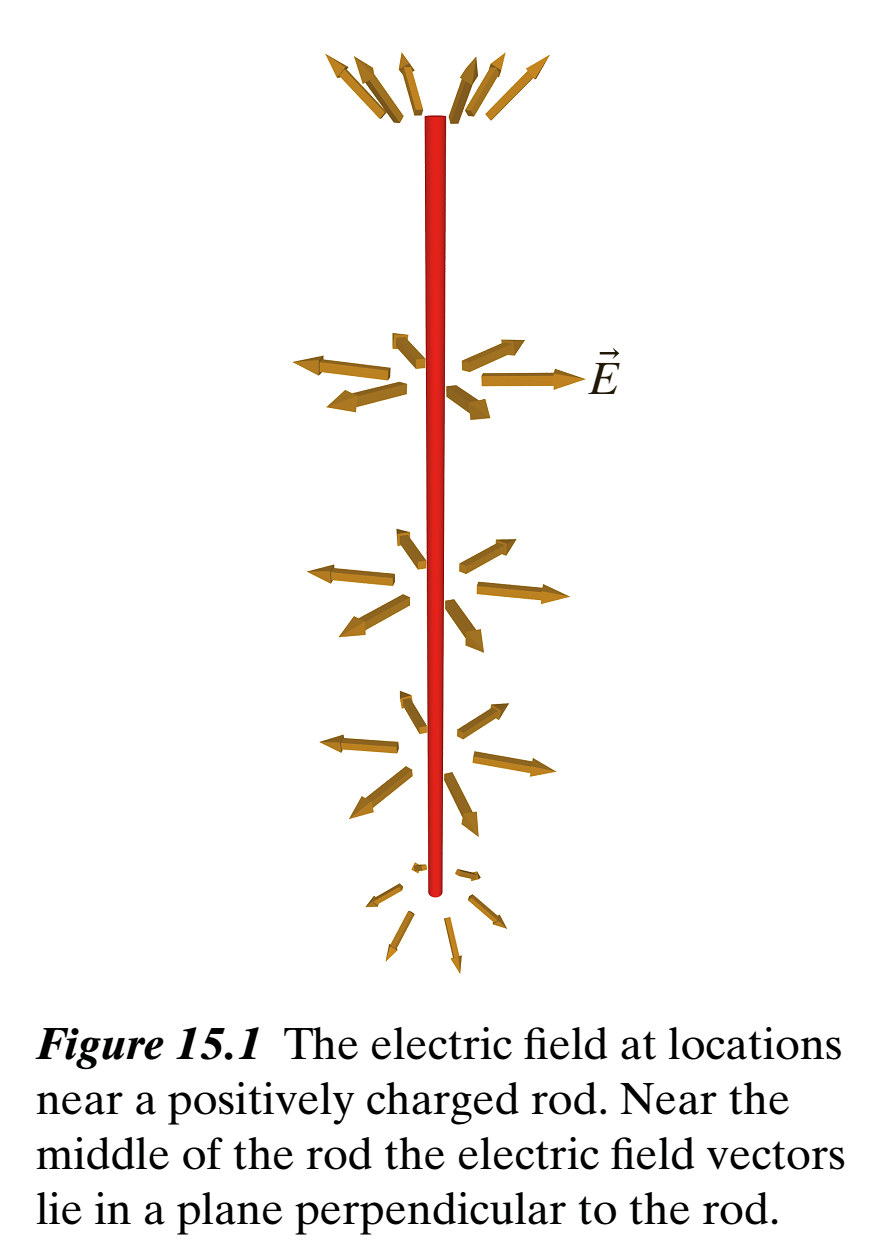
\includegraphics[height=3cm,angle=270]{Efield_wire_matterAndInteractions.PNG}
%\caption{text}
\end{Figure}	


\subsection{Electric Field due to a charged plane}
The magnitude of the electric field due to a large, charged plane is approximately $\frac{Q/A}{2\epsilon_0}$.  (Note that this does not depend on the distance from the plate.)  The direction of the electric field is away (perpendicular) from the plane if the plane is positively charged and towards (perpendicular) the plane if the plane is negatively charged.
\begin{Figure}
\centering
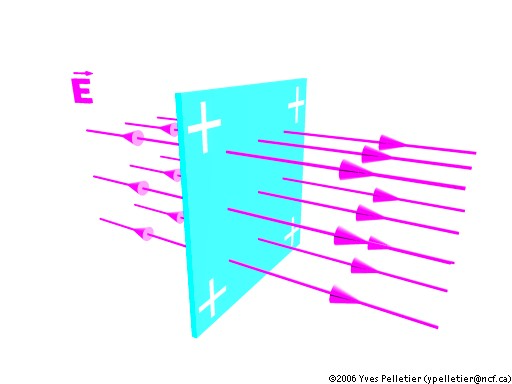
\includegraphics[height=3cm]{eField_plane}
%\caption{text}
\end{Figure}

\section{Electric Force}
The electric field is defined to be the force per charge, $\vec{E} = \vec{F}/q$.

If we know the electric field, this allows us to easily calculate the force $\vec{F}$ felt by a point-like object with net charge $q$, $\vec{F} = q\vec{E}$.

\section{Work and Potential Energy}
The change in potential energy between the start and stop of a path is defined to be negative the work done on that path, or $\Delta U \equiv -W \equiv -\int\vec{F}\cdot\vec{dl}$.  Note that this definition holds no matter what causes the force - gravity or charge.

\section{Electric Potential}
We usually talk about the change in electric potential, $\Delta V \equiv \Delta U / q$.  Note that the definition of $\Delta U$ above means that $\Delta V \equiv -\int\vec{E}\cdot\vec{dl}$.

The integral definition of the electric potential can be turned into a differential definition: $\vec{E} = -\vec{\nabla}{V} = -\frac{\partial V}{\partial x}\hat{x} -\frac{\partial V}{\partial  y}\hat{y} - \frac{\partial V}{\partial z}\hat{z}$.

In some cases we talk about the electric potential at a point in space.  By convention, we mean $V_A = V_A - V_{\inf} = V_A - 0$.

The electric potential at a point a distance $r$ from a point charge $Q$ is $V = \frac{1}{4\pi\epsilon_0}\frac{Q}{r}$.

\section{Energy}
Any region with an electric field $\vec{E}$ is storing energy.  The energy density for this region is $u = \frac{1}{2}\epsilon_0|\vec{E}|^2$.

\section{Vectors}
If point $S$ is located at $(x_1, y_1, z_1)$ and point $P$ is located at $(x_2, y_2, z_2)$ then the vector from point $S$ to point $P$ can be written: $\vec{r} = (x_2 - x_1)\hat{x} + (y_2 - y_1)\hat{y} + (z_2 - z_1)\hat{z}$.  The length of that vector is also called its magnitude and is denoted $|\vec{r}|$, where $|\vec{r}| = \sqrt{(x_2 - x_1)^2 + (y_2 - y_1)^2 + (z_2 - z_1)^2}$.  The magnitude of $\vec{r}$ is sometimes denoted simply by $r$.

\subsection{Unit Vectors}
A unit vector is a vector with magnitude one (``unity'') and is denoted with a hat: $\hat{r} = \vec{r}/|\vec{r}|$.

\subsection{Dot Product}
The dot product between two vectors results in a scaler and measures the ``overlap'' between two vectors.  If two vectors are perpendicular, their dot product is zero.  

\begin{align*}
\vec{a}\cdot\vec{b} &= a_x*b_x + a_y*b_y + a_z*b_z \\
                    &= |\vec{a}||\vec{b}|\cos{\theta}
\end{align*}
                  
Note that $\hat{x}\cdot\hat{x} = 1$ while $\hat{x}\cdot\hat{y} = 0$.

\begin{Figure}
\centering
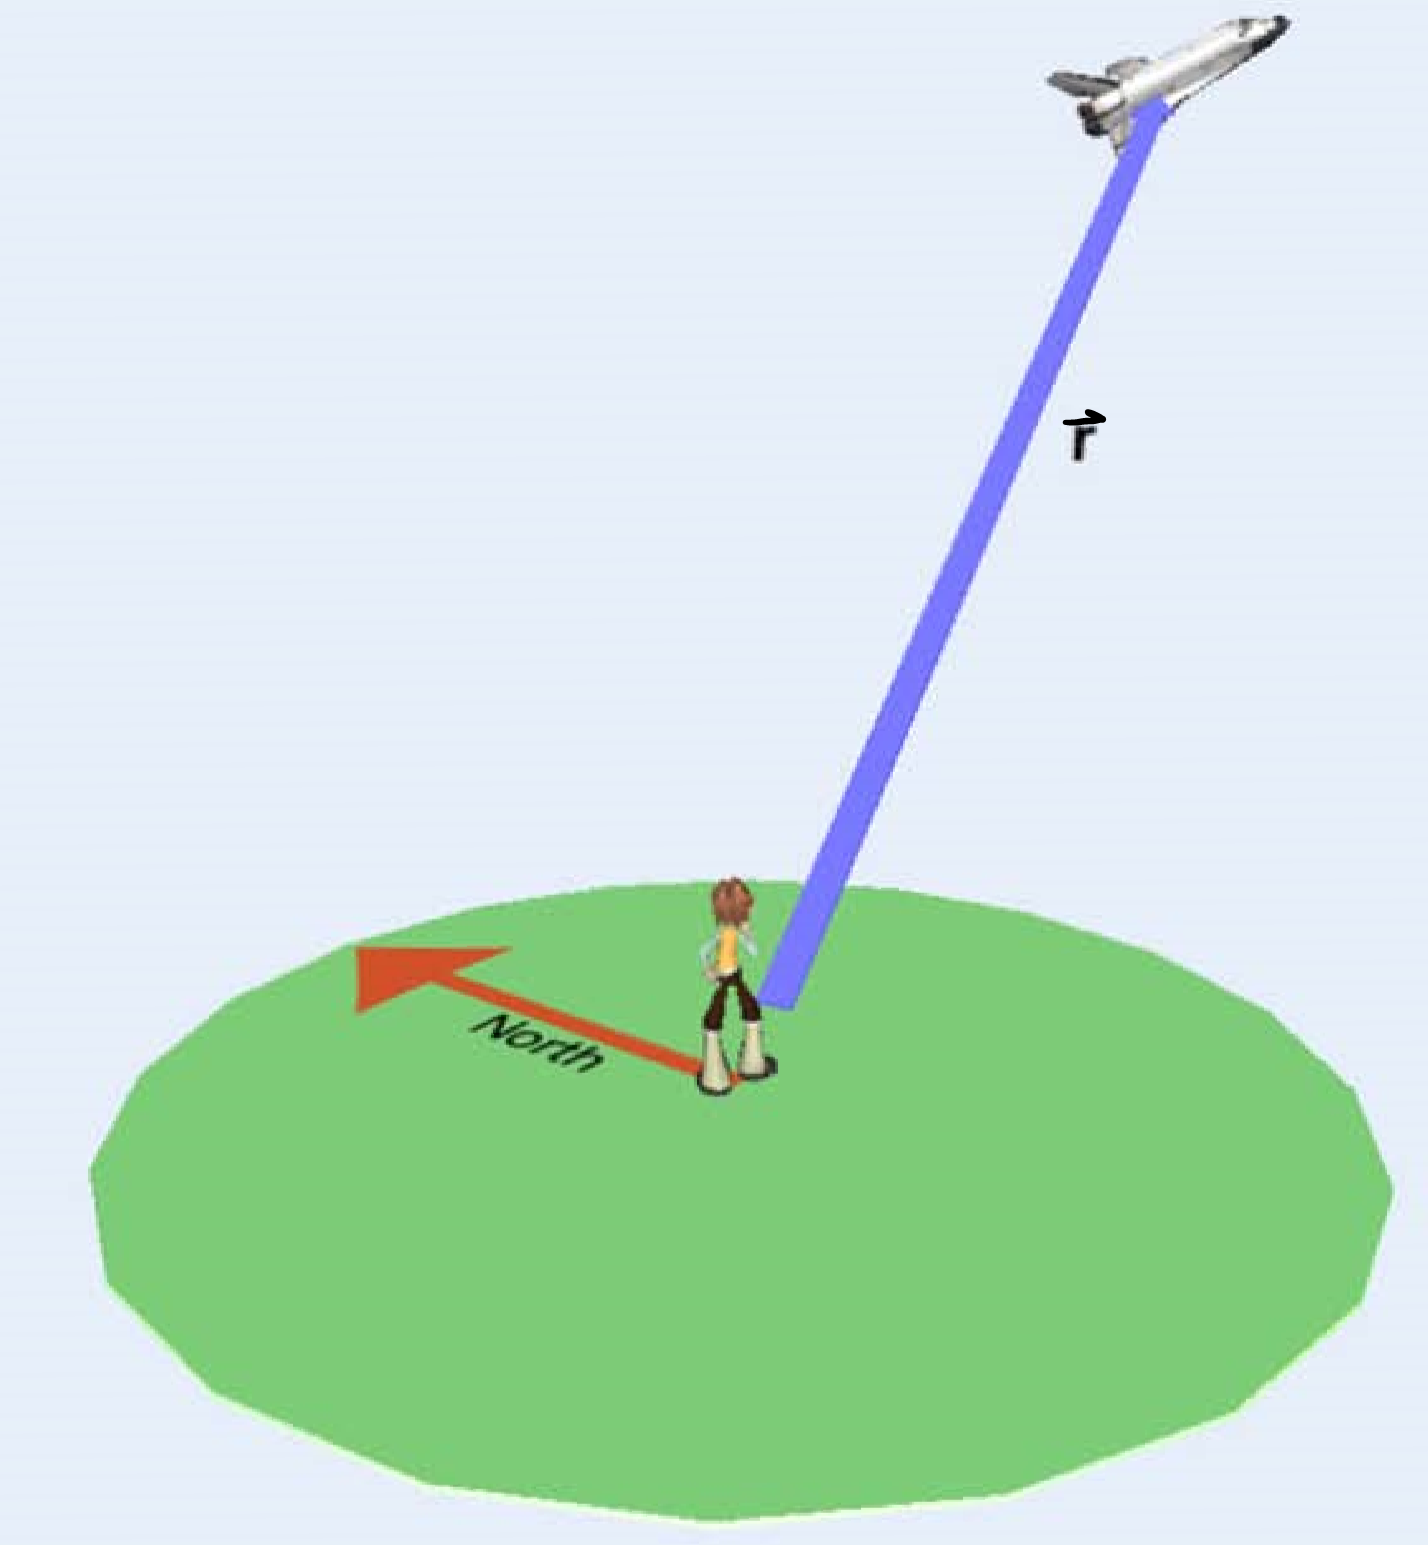
\includegraphics[width=0.9\textwidth]{r_vector.PNG}
%\caption{text}
\end{Figure}

\section{Constants}

$\frac{1}{4\pi\epsilon_0} = 9\times 10^9 N/Cm^2$ \newline
$\epsilon_0 = 8.85\times 10^{-12} {Cm^2/N}$ \newline
charge of an electron (denoted $-e$) = $-1.6\times 10^{-19} C$\newline
charge of a proton (denoted $e$) = $1.6\times 10^{-19} C$\newline
mass of an electron = $9.1\times 10^{-32} kg$ \newline
mass of a proton = $1.673\times 10^{-27} kg$ \newline
acceleration due to gravity (near the Earth's surface) = $9.8 N/kg = 9.8 m/s^2$ \newline
gravitational force constant $G$ = $6.67\times 10^{-11} Nm^2/kg$

% You can even have references
\rule{0.3\linewidth}{0.25pt}
\scriptsize
\bibliographystyle{abstract}
\bibliography{refFile}
\end{multicols}


\end{document}
